\section{Theory}

	\subsection{Electron Spin Resonance}

		Classical concepts can be used to understand electron spin resonance. The magnetic moment of a particle $mu$ precesses about the field at a frequency known as the Larmor frequency when it is placed in a uniform magnetic field of intensity $H 0$. This Larmor frequency is given by:

		$$\omega_0 = \frac{geH_0}{2mc}$$

		where g is the Lande g-factor ($g=1$ for pure orbital momentum and $g=2$ for a free electron spin). In the case of an ion in a crystal, the behaviour is modified by the environment and the g factor may differ from the Lande g-factor. This effective g-factor is known as the spectroscopic splitting factor.
		
		If now an additional weak magnetic field $H_1$ oriented in the x-y plane and rotating about the z axis (in the same direction as the ``Larmor processing'') with an angular frequency $\omega_1$ is introduced, there is a change in energy of the system.

		\begin{enumerate}
			\item For $\omega_1 \neq \omega_0$, the angle between the field $H_1$ and the magnetic moment $\mu$ will continuously change. Thus their average interaction will be zero.
			\item For $\omega_1 = \omega_0$, the angle between the field $H_1$ and the magnetic moment $\mu$ will be constant. Thus their net interaction is effective.
		\end{enumerate}

		This implies a change in the potential energy of the particle in the magnetic field. The change in $\theta$ is the classical analogy to a transition between sublevels with different $m$.

		Imagine that in the quantum perspective, the electron's intrinsic angular momentum ($S$) combines with its orbital angular momentum ($L$) to generate a resultant ($J$). We are aware that there is an equal energy difference between the magnetic sublevels labelled by the magnetic field $H_0$ and $J+1$. If we now introduce a perturbation of the alternating magnetic field $H_1$ with a frequency corresponding to the difference in energy between the levels $(h\nu)$, there will be induced transitions between neighbouring sublevels in accordance with the selection rules $\Delta m = pm 1$ for magnetic dipolar radiation. The prerequisite for resonance is thus:

		$$\Delta D = g\mu_0 H_0 = h\nu_0 = h\nu_1$$

		Where $\nu_1$ is the resonance frequency in cycles per second.

		\begin{figure}[H]
			\centering
			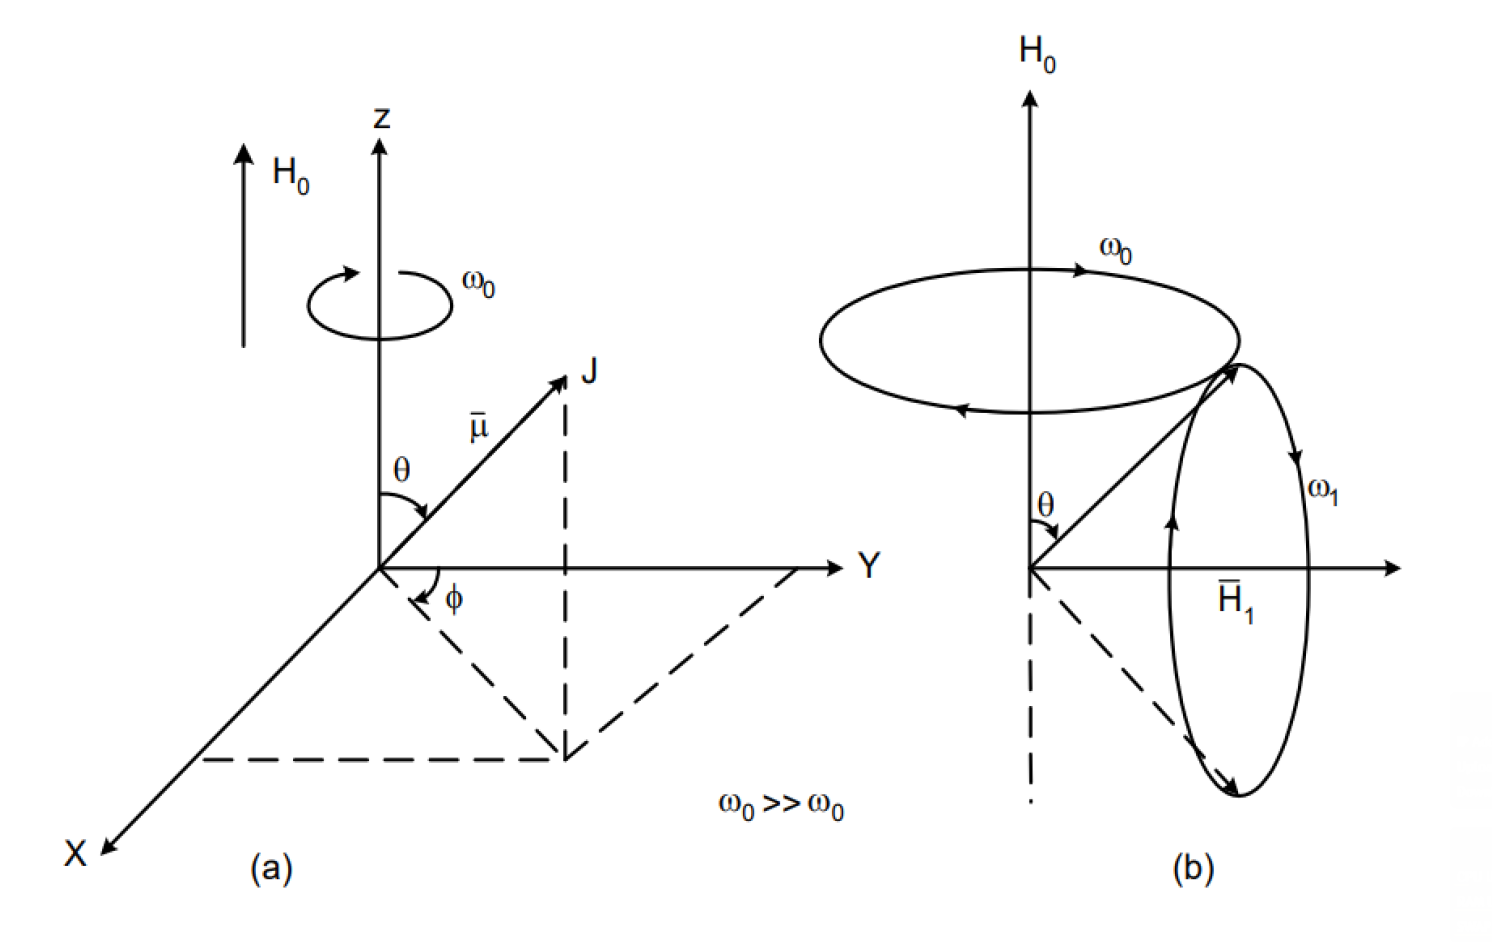
\includegraphics[width=0.5\textwidth]{magnetic_moment}
			\caption{\textbf{(a) Precession of a magnetic moment $\mu_1$ when placed in a magnetic field H0 where in (b) a weak field $H_1$ is applied.}}
			\label{fig:1}
		\end{figure}

	\subsection{Experimental Setup}
	
		The experimental setup consists of four parts:
		\begin{itemize}
			\item \textbf{Basic Circuit:} It is made up of a critically adjusted (marginal) radio frequency oscillator with a frequency range of about 12 to 16 MHz, which is necessary for the oscillation's amplitude to noticeably decrease with even a small increase in load. The DPPH sample kept inside the tank coil is surrounded by a magnetic field created by a Helmholtz coil. An amplitude-modulated carrier is created at resonance and is then detected using a diode detector before being amplified by a chain of three highly stable, low-noise, high-gain audio-frequency amplifiers.
				\begin{figure}[H]
					\centering
					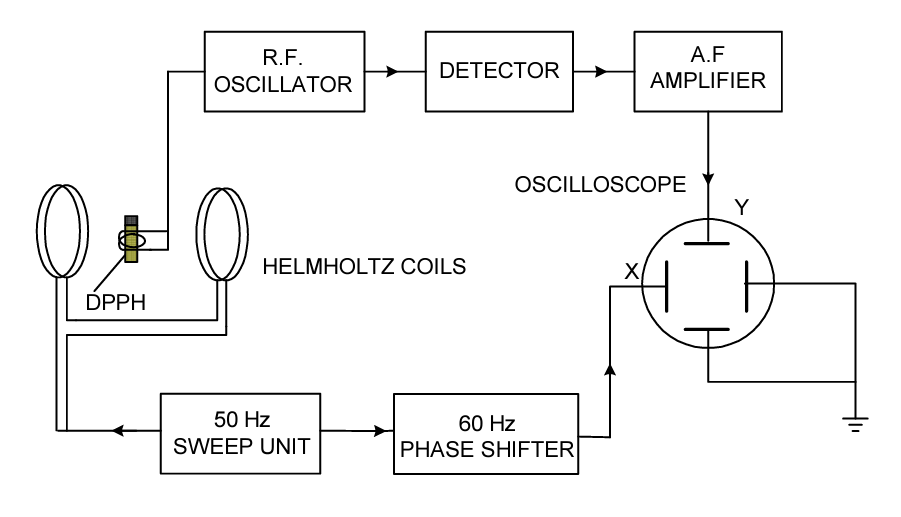
\includegraphics[width=0.5\textwidth]{ESR_Set.png}
					\caption{\textbf{Block diagram of ESR Circuit Setup}}
					\label{fig:2}
				\end{figure}
			\item \textbf{Phase Shifter:} To make it possible to use an ordinary displaying type oscilloscope, instead of a measuring oscilloscope which preserves the phase between X and plate signals, a phase shifter is provided. This can compensate for the phase difference which is introduced in the amplification stage of the ordinary oscilloscope as shown in \hyperref[fig:3]{Figure 3}.
				\begin{figure}[H]
					\centering
					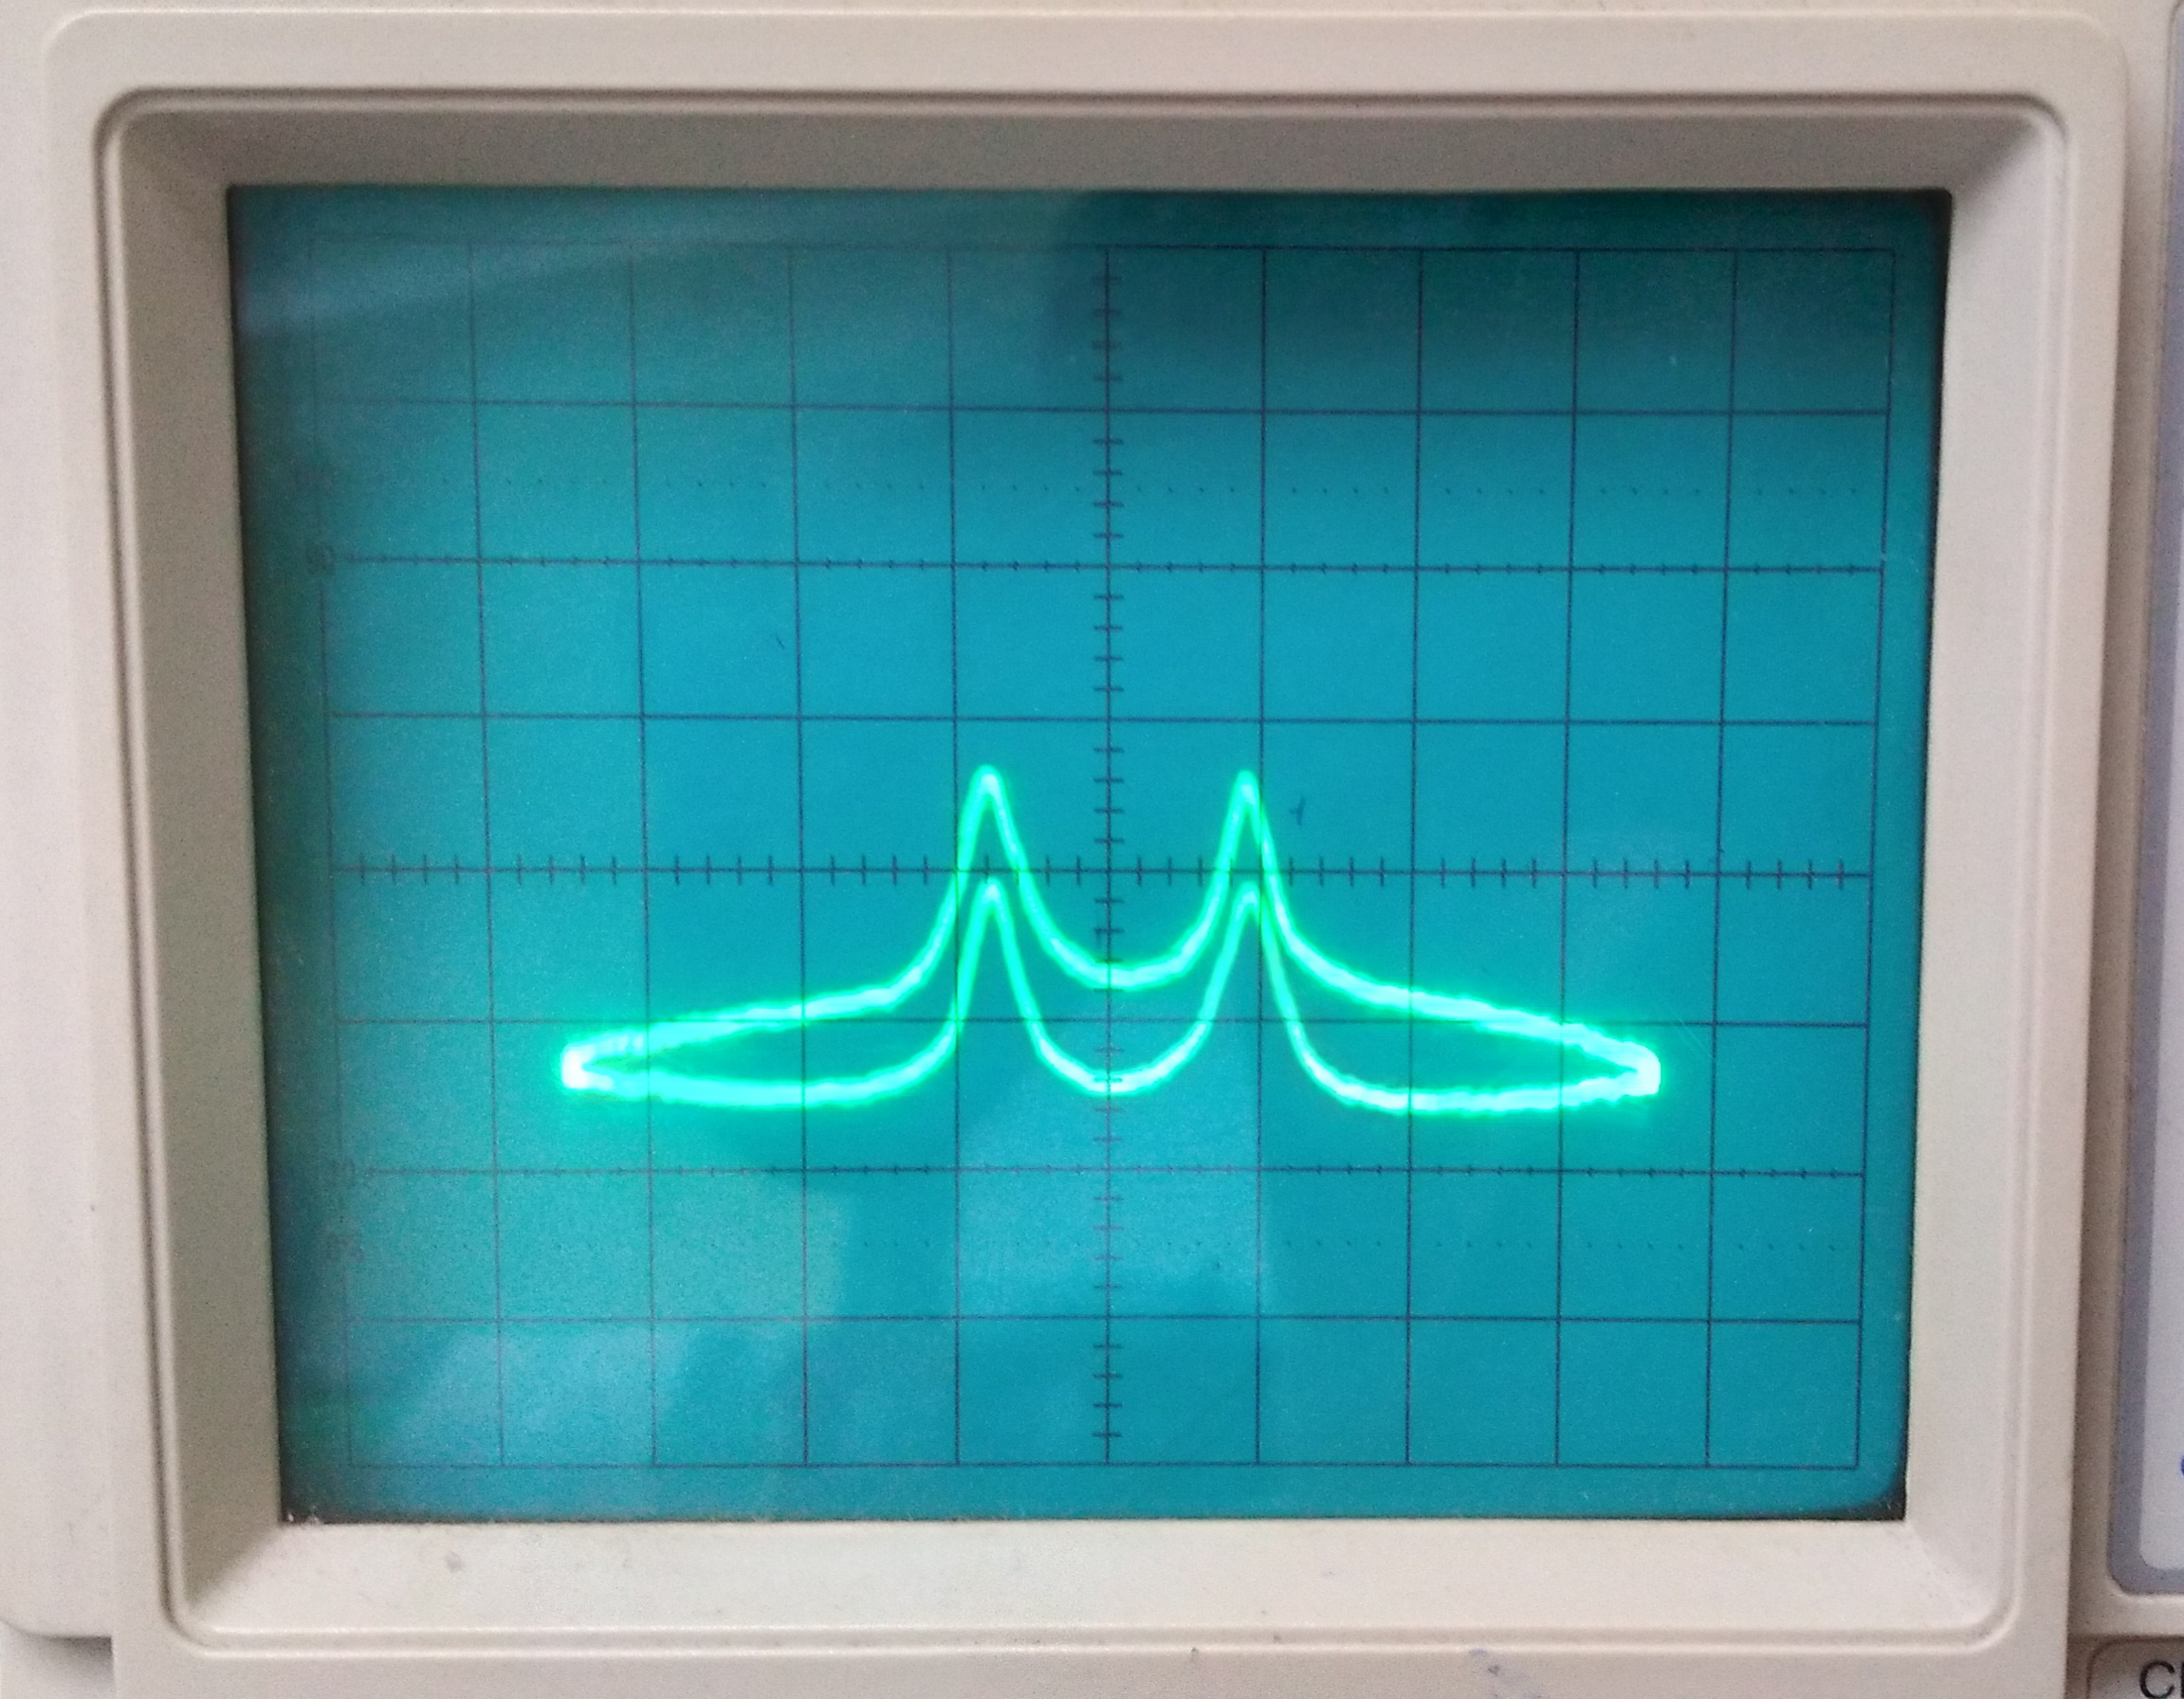
\includegraphics[width=0.4\textwidth]{photo.jpg}
					\caption{\textbf{Oscilloscope}}
					\label{fig:3}
				\end{figure}
			\item \textbf{50Hz Sweep Unit:} For modulation with a low-frequency magnetic field, a 50 Hz current flows through the Helmholtz coils.
			\item \textbf{Power Supplies:} DC Power supply for ESR circuit and the Helmholtz coils power supply consisting of a step-down transformer (220V to 35V AC).
			\item \textbf{Helmholtz Coil} of radius 7.5cm and 500 turns.
		\end{itemize}

	\subsection{Origin of Four Peaks}
	Because the sample absorbs power from the induction coil, oscilloscope output can show peaks that are actually absorption dips. The odd number of amplifying stages in the circuitry is the cause of the peaks. The magnetic field $H_0$, which varies due to an alternating current in the Helmholtz coils, determines the magnitude and direction of the spin precessions with Larmor frequency $omega_0$. Resonance occurs if the radio frequency field is $\omega_1 \approx \omega_0$. The I and II peaks and III and IV peaks will coincide if the X plate signal (50Hz) and Y plate signal (ESR output) are in phase. The coincidence of peaks on the x-scale needs to be calibrated for magnetic field measurements. For magnetic field measurements, the coincidence of peaks on the x-scale must be calibrated. The coincidence guarantees that the magnetic field has maximum values at the ends and zero at the centre. The peaks on the y-scale may not merge completely for a variety of reasons, including 50Hz pickups, power supply ripples, etc.

		\begin{figure}[H]
			\centering
			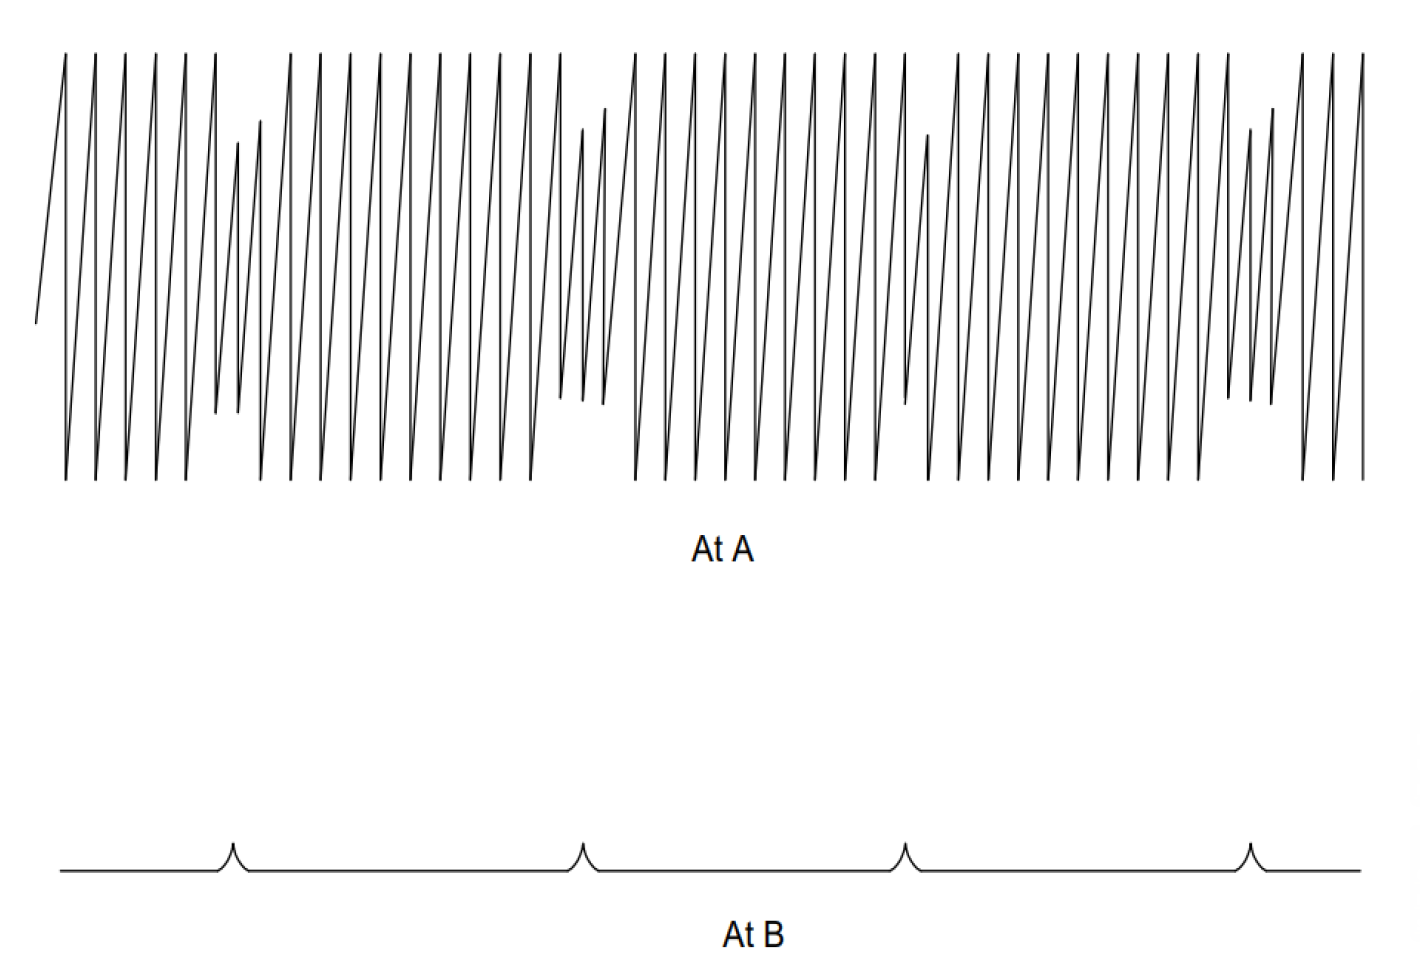
\includegraphics[width=0.5\textwidth]{peaks.png}
			\caption{\textbf{Occurence of Peaks}}
			\label{fig:4}
		\end{figure}

		Therefore g can be calculated by the following equation:

		$$g = \frac{h\nu_0}{\mu_0 H_0}$$

		here $h\;(=6.625\times 10^{-27} erg\;sec$) is the Plack's constant and $\mu_0\;(=0.927\times 10^{-20} erg/Gauss)$ is the permeability of free space.

		$$H_0 = H_{pp}\frac{Q}{P}$$

		Where $H_{pp}$ is the peak-to-peak value of the magnetic field, $Q$ is half the distance between the two peaks and $P$ is the maximum $X$ deflection. A magnetic field defined for RMS field H as:

		$$H_{pp} = 2\sqrt{2}H$$

		H, the RMS magnetic field between the Helmholtz coils is given by:

		$$H = \frac{32\pi nI}{10a\sqrt{125}}$$

		Putting appropriate values in the above equations, we get:

		\begin{equation}
			g = c\times \frac{\nu_0}{IQ} = 3.375\times 10^{-8} \times \frac{\nu_0}{m}
			\label{eq:1}
		\end{equation}

		where $c = \frac{5a\sqrt{125}}{32\pi n \sqrt{2}}\times\frac{Ph}{\mu_0} = 3.375\times 10^{-8}$ and $m$ is the slope of $Q$ vs $\frac{1}{I}$ graph.
